\documentclass[12pt,a4wide,openany]{memoir}







\usepackage{graphicx}
\usepackage{multicol}
\usepackage{afterpage}
\usepackage[pagecolor=none]{pagecolor}
\usepackage{verse}
\usepackage{polyglossia}
\usepackage{fontspec}
\usepackage{url}
\usepackage{titlesec}

\settypeblocksize{20cm}{16cm}{*}
% \setlrmargins{1.5cm}{*}{*}
\usepackage{titlesec}
\titleformat{\chapter}[display]
{\normalfont%
    \Large% %change this size to your needs for the first line
    \bfseries}{\chaptertitlename\ \thechapter}{20pt}{%
    \Large %change this size to your needs for the second line
    }

\setdefaultlanguage{english}

\setotherlanguage[numerals=hebrew]{hebrew}

\fontspec [Path = /Users/scott/Library/Fonts/culmus/ ,UprightFont = *Regular,  BoldFont      = *Demi-Bold]{Shofar}
\fontspec [Path = /Users/scott/Library/Fonts/culmus/ ,UprightFont = *-Regular,  BoldFont      = *-Bold]{HadasimCLM}
\fontspec[Path = /usr/local/texlive/2017/texmf-dist/fonts/truetype/typoland/carlito/, 
UprightFont = *-Regular,
BoldFont = *-Bold,
ItalicFont = *-Italic ]{Carlito}


\newfontfamily\hebrewfont[Script=Hebrew]{Hadasim CLM}
%
%\setmainfont{Carlito}[%
% Path = /usr/local/texlive/2017/texmf-dist/fonts/truetype/typoland/carlito/ ,% 
% UprightFont = *-Regular,
% BoldFont = *-Bold,
% ItalicFont = *-Italic ]

% \setmainfont[%
%  Path = /Users/scott/Library/Fonts/cabin/ ,% 
%  UprightFont = Cabin-Regular.otf,
%  BoldFont = *-Bold,
%  ItalicFont = *-RegularItalic ]{Cabin}

\setmainfont[ Path =
/usr/local/texlive/2017//texmf-dist/fonts/opentype/impallari/quattrocento/ ]{Quattrocento}
%\setmainfont[ Path =
%/usr/local/texlive/2017//texmf-dist/fonts/opentype/catharsis/cormorantgaramond/]{Cormorant Garamond}
\setmainfont[ Path =
/usr/local/texlive/2017//texmf-dist/fonts/opentype/impallari/raleway/ ,
 UprightFont = Raleway-Regular.otf,
 BoldFont = Raleway-Bold,
 ItalicFont = Raleway-Regular-Italic ] {Raleway}
\setmainfont[ Path =
/usr/local/texlive/2017//texmf-dist/fonts/opentype/catharsis/cormorantgaramond/ ,
 UprightFont = CormorantGaramond-SemiBold.otf,
 BoldFont = CormorantGaramond-Bold,
 ItalicFont = CormorantGaramond-SemiBoldItalic ] {Cormorant Garamond}
%\setmainfont{Georgia}


%\setmainfont{Palatino}

\titleformat{\chapter}[display]
{\normalfont%
    \Large% %change this size to your needs for the first line
    \bfseries}{\chaptertitlename\ \thechapter}{20pt}{%
    \Large %change this size to your needs for the second line
    }




\newcommand{\HgSource}[1]{\hfill{\small---\itshape{#1}}}
\newcommand{\HgEllipsis}{\ensuremath{\left[\ldots\right]}}
\newcommand{\HgHL}[1]{{\large\textbf{#1}\par\noindent\\[-.5em]}}
\newcommand{\HgFill}{\vfill \hrule \vfill}
\newcommand{\HgInst}[1]{{\noindent\sffamily{\bfseries{#1}}}}
\newcommand{\LSrc}{\textsuperscript{\upshape{[L]}}}
\newcommand{\cH}{Ch}
\newcommand{\CH}{CH}
\newcommand{\ch}{ch}
%\d{H}


\newenvironment{HgHebrew}{\begin{hebrew}\strut\\\noindent\Large}{\end{hebrew}}
\newenvironment{HgHebrewl}{\begin{hebrew}\strut\\\noindent\large}{\end{hebrew}}
\newenvironment{HgEnglish}{\strut\\\noindent}{\vspace{1em}}
\newenvironment{HgTranslit}{\strut\\\noindent\begin{itshape}}{\end{itshape}\vspace{1em}}
\newenvironment{myitemize}[0]{%
        \protect\begin{itemize}%
        \vspace*{-2mm}%
        \setlength{\topsep}{-6pt}%
        \setlength{\labelsep}{4pt}%
        \setlength{\partopsep}{-6pt}%
        \setlength{\itemsep}{-2pt}}%
{\protect\end{itemize}}


\newenvironment{myenumerate}[0]{%
        \protect\begin{enumerate}%
        \vspace*{-2mm}%
        \setlength{\topsep}{-6pt}%
        \setlength{\labelsep}{4pt}%
        \setlength{\partopsep}{-6pt}%
        \setlength{\itemsep}{-2pt}}%
{\protect\end{enumerate}}

\title{\vspace*{-4cm}Haggadah}

\author{\vspace*{-1cm}Seder for the perplexed \& perplexing family}
\date{Pesach, 5778}

\usepackage{tocloft}
\setlength{\cftbeforechapterskip}{.1ex}
%\setlrmargins{2cm}
\begin{document}
\frontmatter
\newpagecolor{red!75!green!50!blue!25}\afterpage{\restorepagecolor}
\pagenumbering{roman}
\maketitle
\thispagestyle{empty}



\noindent\hspace*{-5cm}
\vspace*{-3cm}
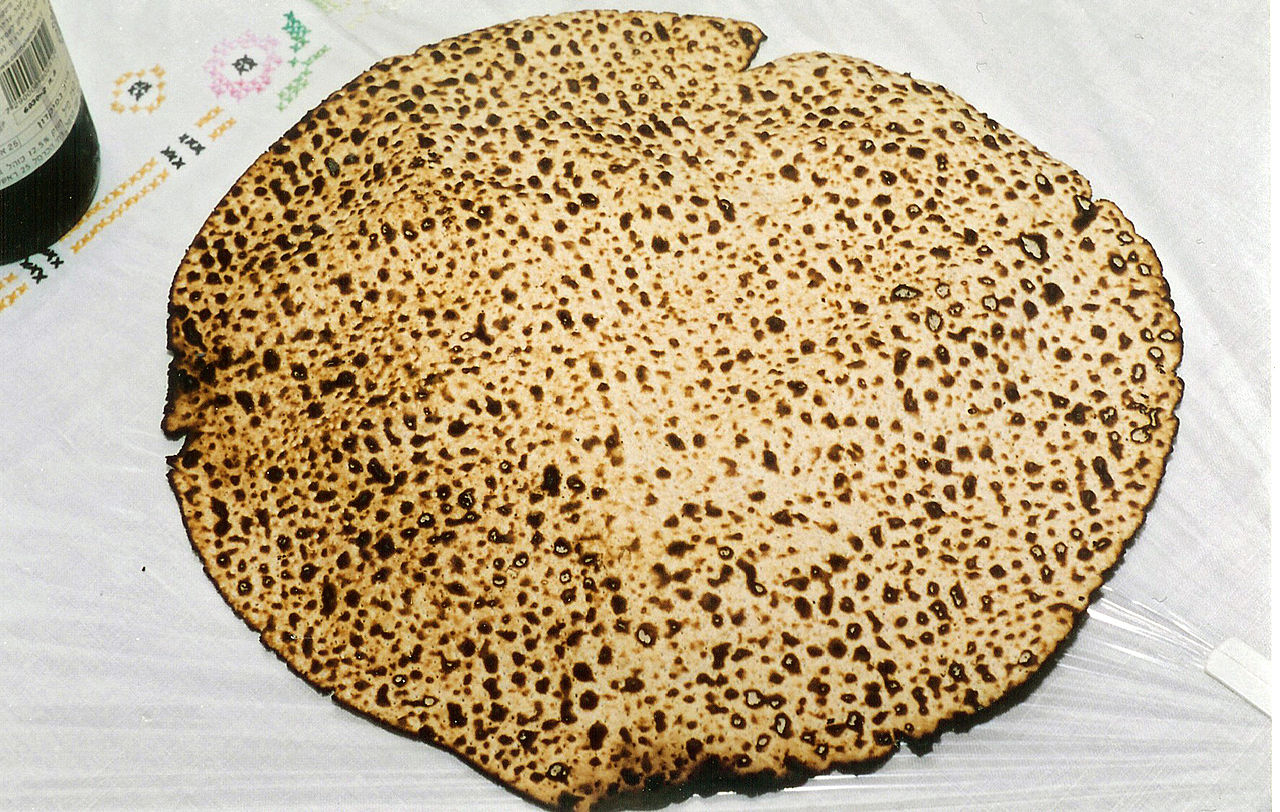
\includegraphics[width=232mm]{figs/matzo.jpg}
\thispagestyle{empty}

%\newpage


\newpage

\phantom{Deliberately blank}
\thispagestyle{empty}

\newpage
\setcounter{page}{1}
\maketitle

\newpage
\vfill\phantom{Hello}\vfill

\vfill
\paragraph*{Acknowledgments}

\begin{itemize}
\item Major  source material for this haggadah was the {\LaTeX}
  source of the The Columbia Commune Churchill Free Haggadah
  \url{https://github.com/jacobandreas/haggadah}, which had been
  placed in the public domain.
\item The photo on the
  front cover is by Yoninah (Own work) [GFDL
  (\url{http://www.gnu.org/copyleft/fdl.html}), CC-BY-SA-3.0
  (\url{http://creativecommons.org/licenses/by-sa/3.0/}) or CC BY 2.5
  (\url{http://creativecommons.org/licenses/by/2.5)}], via Wikimedia
  Commons
\end{itemize}

\vfill
\noindent
This  haggadah is produced in {\XeLaTeX}. The English text is
set in Charter. The Hebrew text is set in Shofar.

\newpage


\chapter{The Passover seder}

\vfill

\vspace{-2em}
\begin{HgHebrew}
  \begin{center}
  קדש 
  -
  ורחץ
  -
  כרפס 
  -
  יחץ 
  -
  מגיד 
  -
  רחצה 
  -
  מוציא
  -
  מצה 
  \\
  מרור 
  -
  כורך 
  -
  שולחן עורך 
  -
  צפון
  -
  ברך 
  -
  הלל 
  -
  נירצה 
  \end{center}
\end{HgHebrew}
\vspace{-3em}
\begin{HgTranslit}
  \begin{center}
  {\small 
    KADESH - UR{\CH}ATZ - KARPAS - YA{\CH}ATZ - % \\
    MAGID - RA{\CH}TZA - MOTZI - MATZAH \\ 
    MAROR - KOREI{\CH} - SHUL{\CH}AN OREI{\CH} - % \\
    TZAFUN - BAREI{\CH} - HALLEL - NIRTZAH}
  \end{center}
\end{HgTranslit}



\newpage


\tableofcontents*

\newpage
\setcounter{page}{1}
\pagenumbering{arabic}


\chapter{Kiddush}

\vspace*{-3cm}

\noindent
On Shabbat

\begin{center}
\begin{tabular}{r}
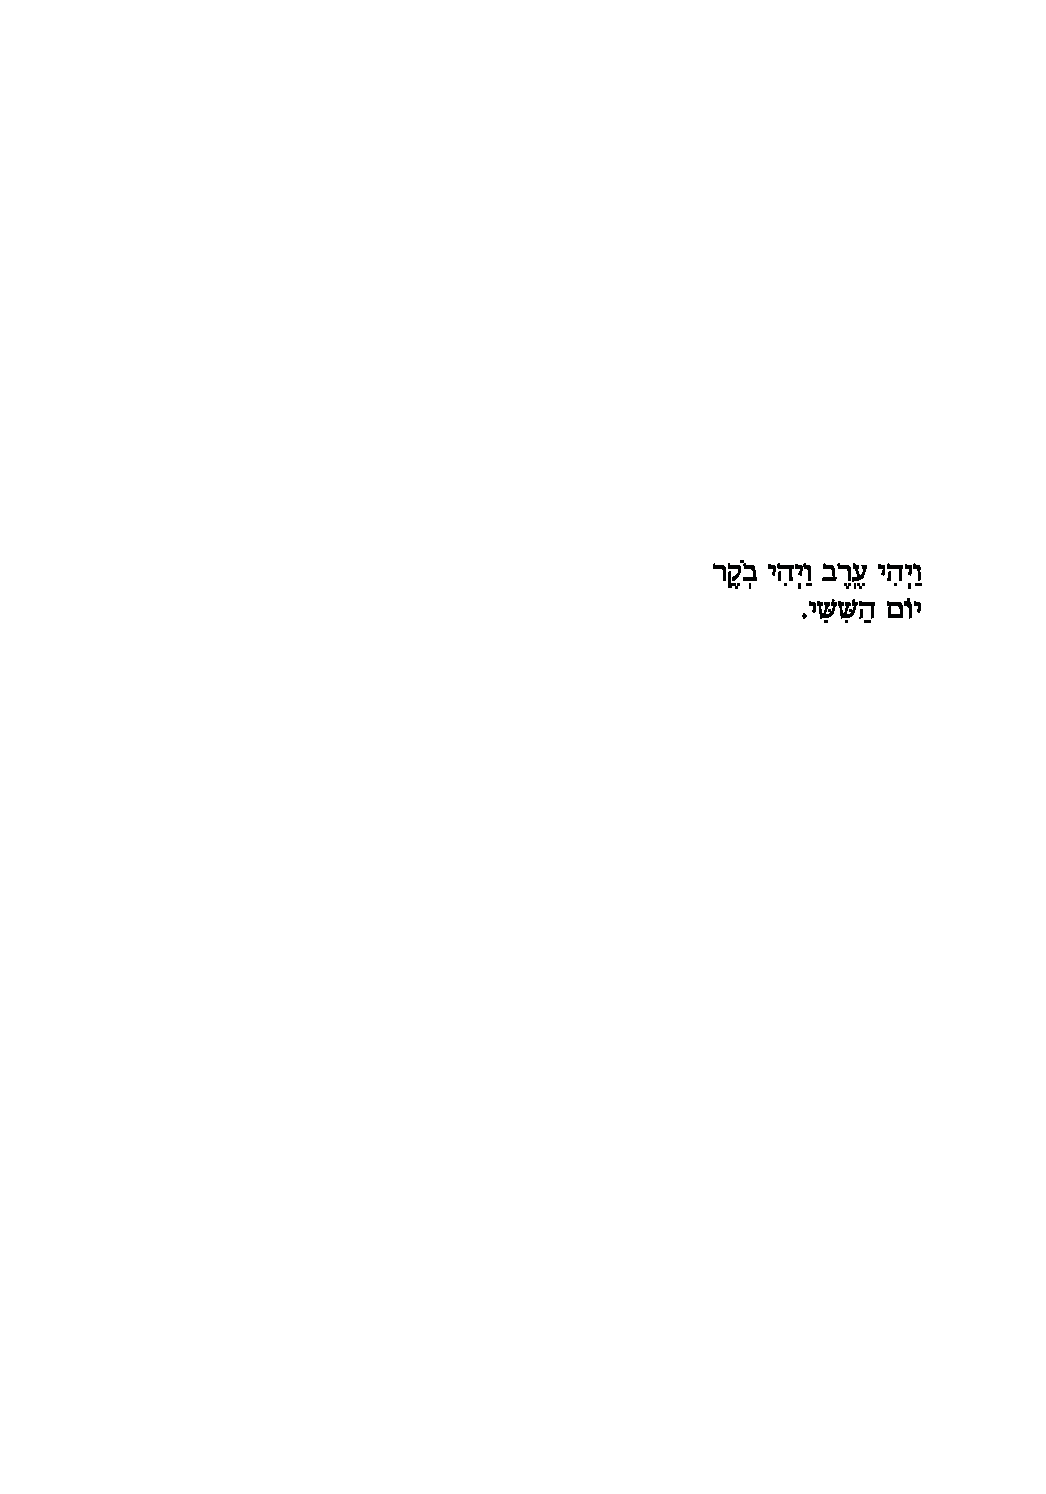
\includegraphics[width=2cm,trim=25mm 0mm 0mm 0mm]{figs/0A010-vayehi}\\
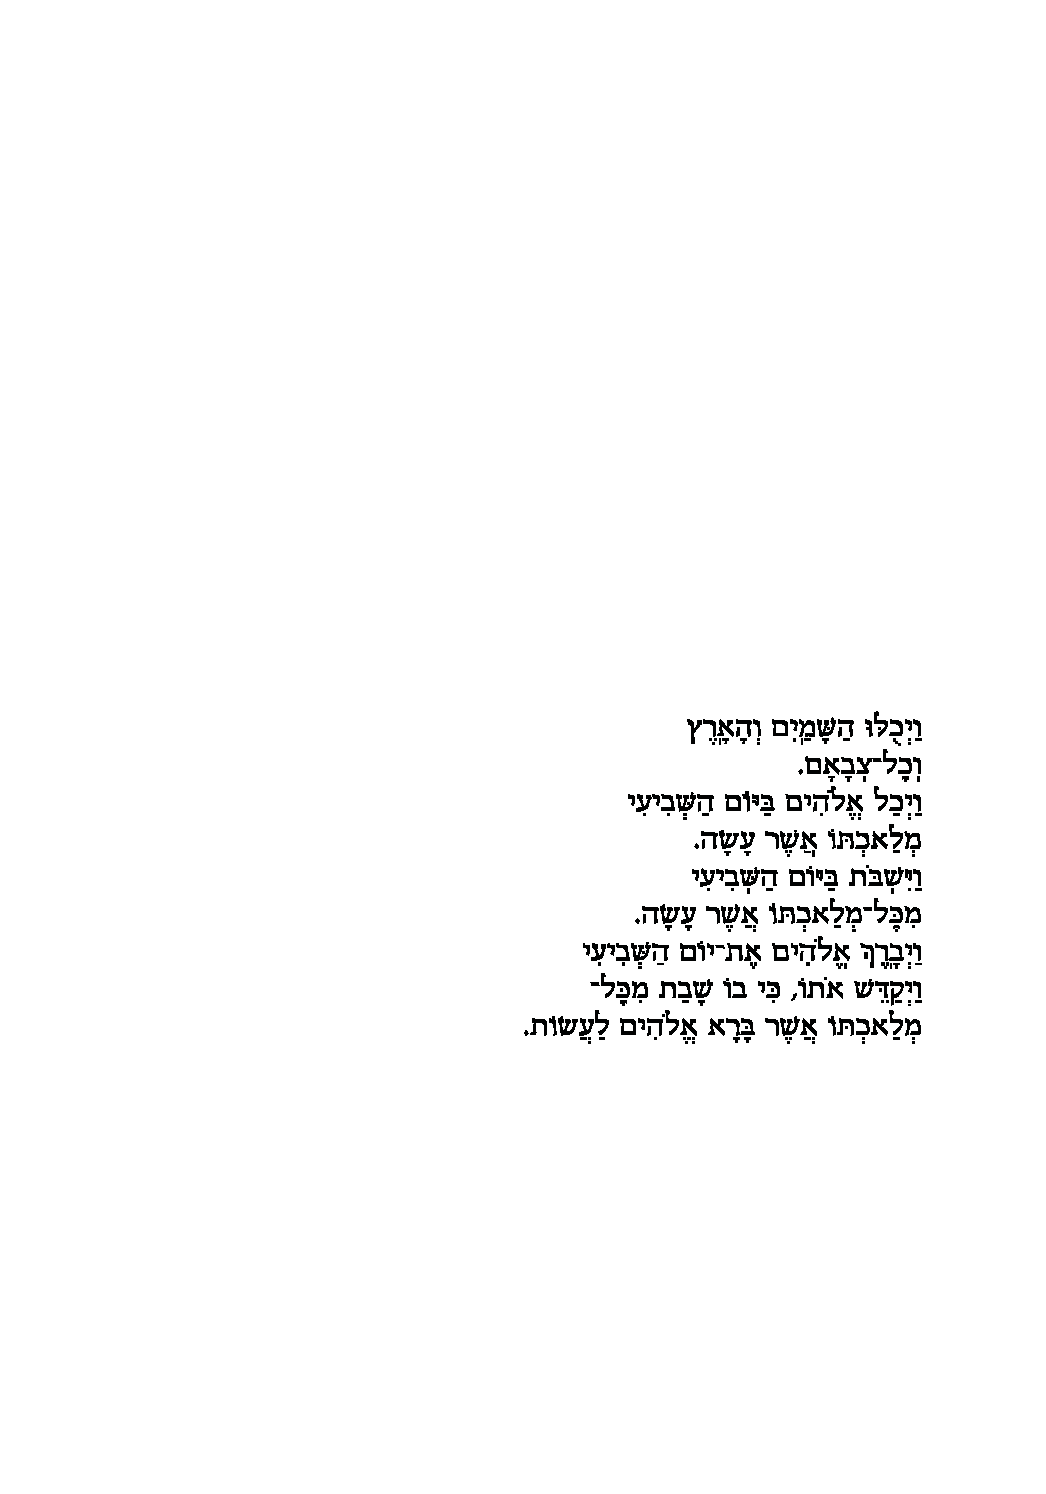
\includegraphics[width=9cm,trim=0mm 0mm 2mm 0mm,clip]{figs/0A014-vayechulu}\\
\end{tabular}
\end{center}

\newpage
\HgInst{Pour the first cup of wine, and read:}

\begin{tabular}{r}
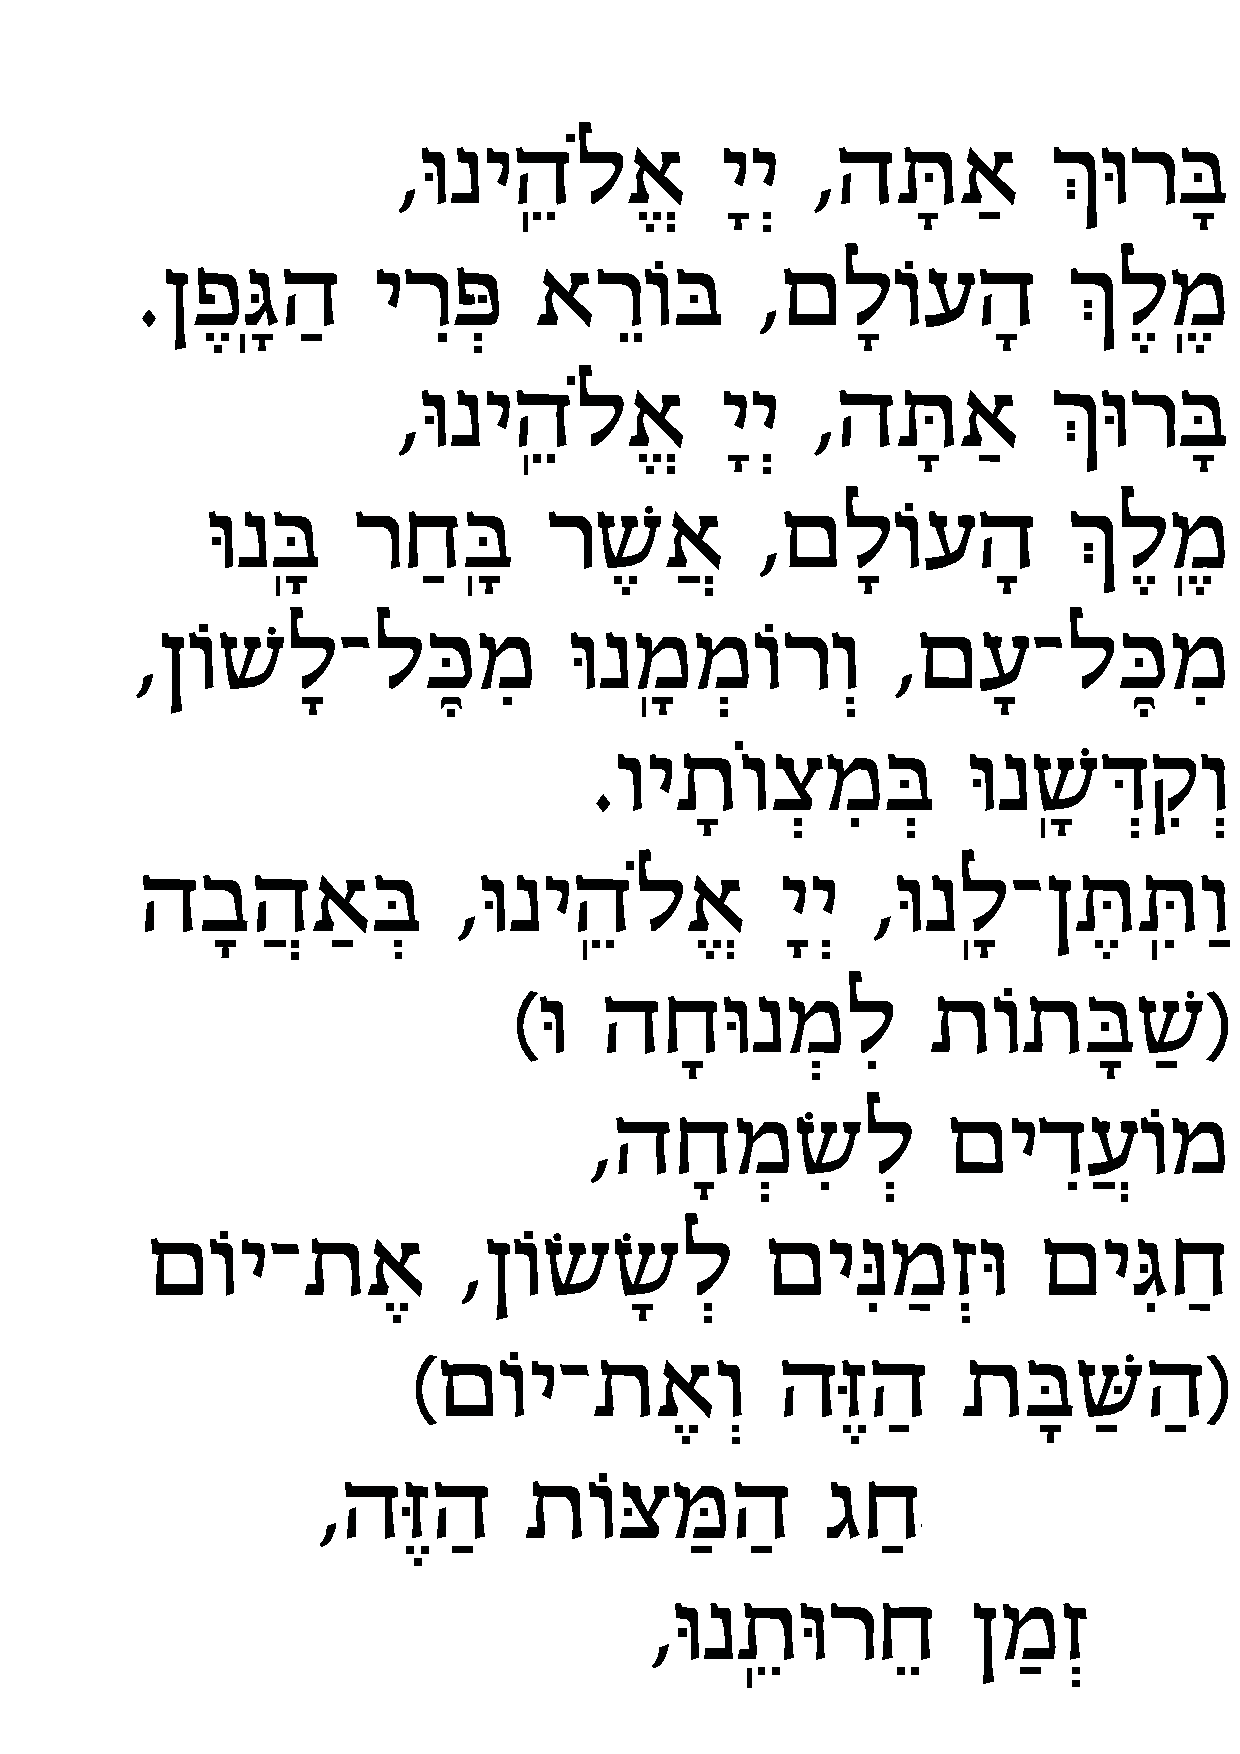
\includegraphics[width=9cm,trim=0 16mm 0 0]{figs/0A020-kiddush1}\\
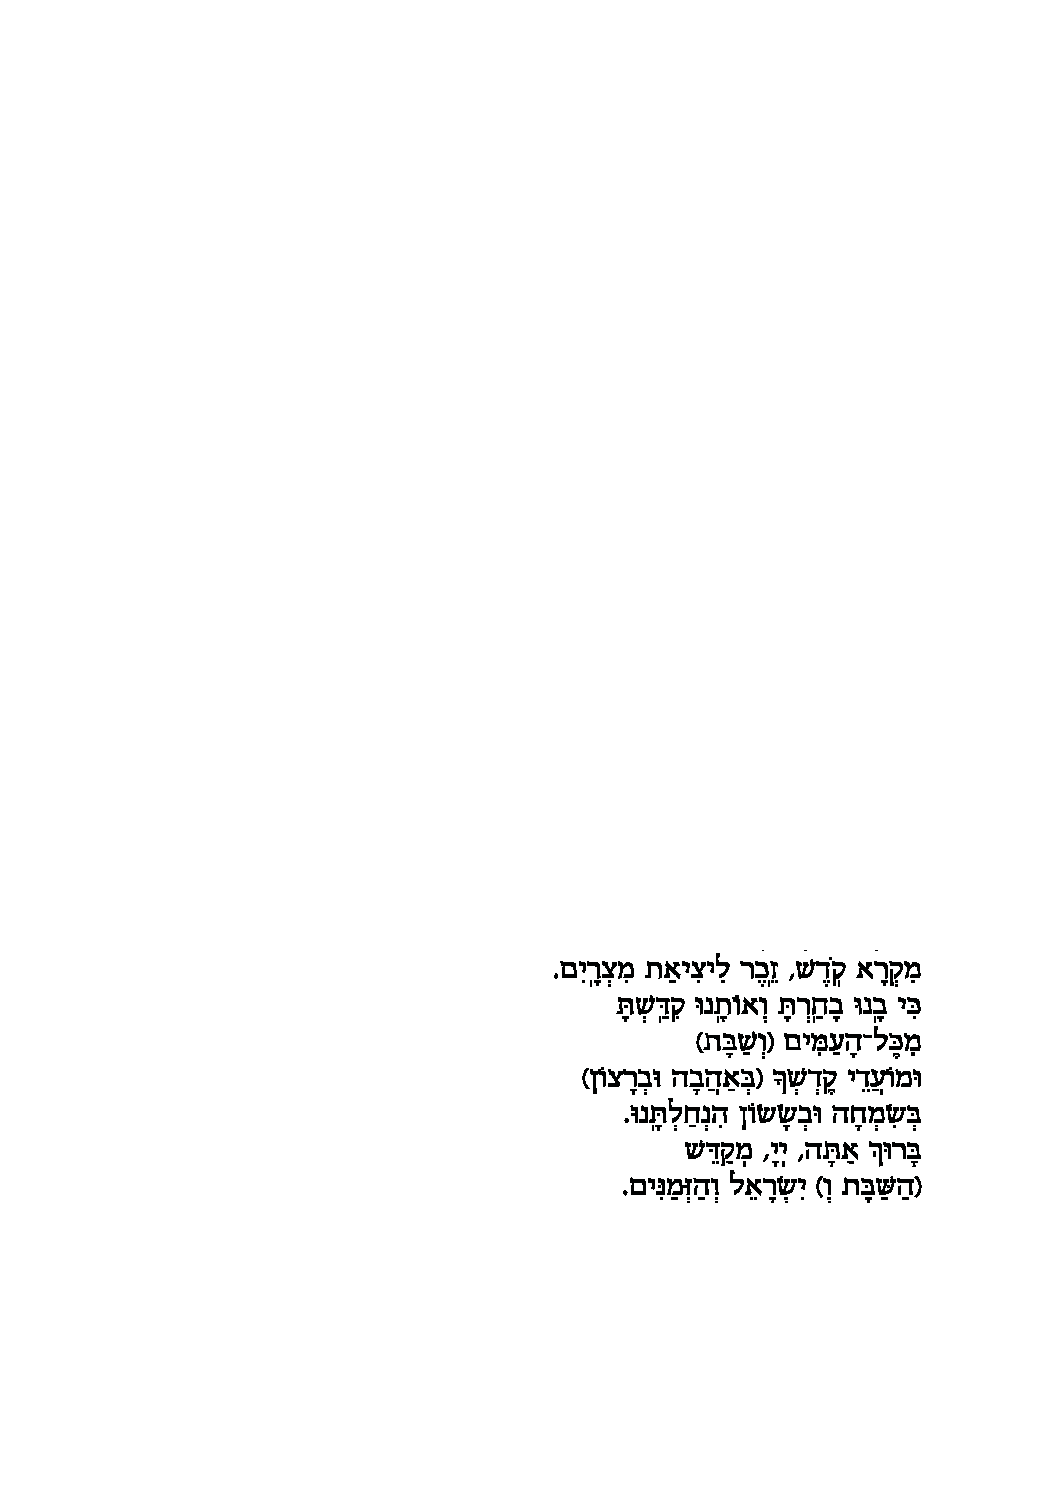
\includegraphics[width=9cm]{figs/0A024-kiddush2}\\
\end{tabular}


\newpage

\paragraph*{Shehecheyanu}

\begin{HgHebrew}
 בָּרוּךְ אַתָּה אֲדֹנָי אֱלֹהֵינוּ מֶלֶךְ הָעוֹלָם,
 שֶׁהֶחֱיָנוּ וְקִיְּמָנוּ וְהִגִּיעָנוּ לַזְּמָן הַזֶּה.
\end{HgHebrew}


\begin{HgTranslit}
Baruch atah Adonai, Eloheinu Melech haolam,
shehecheyanu, v'kiy'manu, v'higianu laz'man hazeh.
\end{HgTranslit}

\begin{HgEnglish}
Our praise to You, Adonai, Sovereign of all:
for giving us life, sustaining us, and enabling us to reach this season.
\end{HgEnglish}

\noindent
\HgInst{Drink the first cup of wine}

\vfill


\chapter{Ur{\ch}atz: Washing the hands}


\HgInst{Those who wish to may wash your hands, without reciting a blessing.}


\vfill

\newpage

\chapter{Karpas: The green vegetable}

\begin{HgEnglish}\raggedright
  The green vegetable represents rebirth, renewal and growth. The salt
  water represents the tears we shed when we were slaves in Egypt. The
  karpas is usually a fresh vegetable like parsley, watercress or
  celery, though there are other customs.
\end{HgEnglish}

\vfill

\HgInst{Distribute the karpas, and dip them in saltwater.}

\begin{HgHebrew}
  בָּרוּךְ אַתָּה יי אֱלֹהֵינוּ מֶלֶךְ הָעוֹלָם, 
  \\
  בּוֹרֵא פְּרִי הָאֲדָמָה.

%ברוך אתה יי אלהינו מלך העולם, 
%  \\
%  בורא פרי האדמה.
\end{HgHebrew}

\begin{HgTranslit}
  Baru{\ch} atah Adonai, eloheinu mele{\ch} ha'olam, \\
  borei p'ri ha'adamah.
\end{HgTranslit}
\vspace{-1em}
\begin{HgEnglish}
  Blessed are you, Adonai, Sovereign of the Universe, \\
  Who creates the fruit of the earth.
\end{HgEnglish}

\HgInst{Eat the karpas.}

\vfill

\newpage
\chapter{Ya{\ch}atz: Breaking the matzah}
\vfill

\HgInst{Break the middle matzah, and set aside the larger piece as the
afikoman.}

\HgInst{Hold the remaining matzah up, and read:}

\vfill
\newpage
\begin{HgEnglish}
  \textbf{
  This is the bread of affliction that our ancestors ate
  in the land of Egypt.
  }
  All who are hungry, come and eat; \\
  all who are needy, come and celebrate the Passover. \\
  Now we are here;
  next year may we be in Israel; \\
  now we are slaves;
  next year may we be free.
\end{HgEnglish}

\begin{HgHebrew}
  הָא לַחְמָא עַנְיָא דִּי אֲכָלוּ אַבְהָתָנָא
  \\
  בְּאַרְעָא דְמִצְרָיִם.
  \\
  כָּל דִּכְפִין יֵיתֵי וְיֵכוֹל,
  \\
  כָּל דִּצְרִיךְ יֵיתֵי וְיִפְסַח. 
  \\
  הָשַּׁתָּא הָכָא,
  לְשָׁנָה הַבָּאָה בְּאַרְעָא דְיִשְׂרָאֵל.
  \\
  הָשַּׁתָּא עַבְדֵי,
  לְשָׁנָה הַבָּאָה בְּנֵי חוֹרִין.
\end{HgHebrew}

\begin{HgTranslit}
  Hala{\ch}ma anya di a{\ch}alu avhatana \\
  b'ara d'mitzrayim.
  Kol di{\ch}fin yeitei v'ye{\ch}ol \\
  kol ditzri{\ch} yeitei v'yifsa{\ch}. \\
  Hashata ha{\ch}a, %\\
  l'shanah haba'ah b'ara d'yisrael. \\
  Hashata avdei, %\\
  l'shanah haba'ah b'nei {\ch}orin.
\end{HgTranslit}


\vfill

\HgInst{Pour (but not drink!) the second cup of wine.}

\vfill

\newpage

\chapter{Magid: The Passover story}

\subsubsection*{The  four questions.}

\vfill

\HgInst{The youngest person present  (however defined, or next in
  turn) recites:}

\vfill

\begin{HgEnglish}
  \HgHL{Why is this night different from all other nights?}
  On other nights, we eat leavened bread and matzah; tonight only matzah. \\
  On other nights, we eat all kinds of herbs; tonight bitter herbs. \\
  On other nights, we do not dip our food; tonight we dip twice. \\
  On other nights, we eat upright or reclining; tonight we all recline. \\
\end{HgEnglish}

\begin{HgHebrew}
מַה נִּשְּׁתַּנָה הַלַּיְלָה הַזֶּה מִכָּל הַלֵּילוֹת? 
\\
שֶׁבְּכָל הַלֵּילוֹת אָנוּ אוֹכְלִין חָמֵץ וּמַצָּה,
%\\
הַלַּיְלָה הַזֶּה כּוּלוֹ מַצָּה. 
\\
שֶׁבְּכָל הַלֵּילוֹת אָנוּ אוֹכְלִין שְׁאָר יְרָקוֹת,
%\\
הַלַּיְלָה הַזֶּה מָרוֹר. 
\\
שֶׁבְּכָל הַלֵּילוֹת אֵין אֶנוּ מַטְבִּילִין אֲפִילוּ פַּעַם אֶחָת, 
%\\
הַלַּיְלָה הַזֶּה שְׁתֵּי פְעָמִים. 
\\
שֶׁבְּכָל הַלֵּילוֹת אָנוּ אוֹכְלִין בֵּין יוֹשְׁבִין וּבֵין מְסֻבִּין, 
%\\
הַלַּיְלָה הַזֶּה כֻּלָנו מְסֻבִּין. 
\end{HgHebrew}

\begin{HgTranslit}
  \HgHL{Ma nishtanah halailah hazeh mikol haleilot?}
  Shebe{\ch}ol haleilot, anu o{\ch}lin {\ch}ametz umatzah, 
  halailah hazeh kulo matzah. \\
  Shebe{\ch}ol haleilot, anu o{\ch}lin sh'ar y'rakot, 
  halailah hazeh maror. \\
  Shebe{\ch}ol haleilot, ein anu matbilin afilu p'am e{\ch}ad,
  halailah hazeh sh'tei f'amin. \\
  Shebe{\ch}ol haleilot, anu o{\ch}lin bein yoshvin uvein m'subin,
  halailah hazeh \\ \strut $\quad$ kulanu m'subin.
\end{HgTranslit}

\vfill

\newpage

\HgInst{Uncover the matzah, and read:}

\begin{HgEnglish}
We were slaves of Pharaoh in Egypt, and our God brought us out from there
with a mighty hand and an outstretched arm.
Now, if God had not brought our ancestors out from Egypt, then we, our
children, and our children's children might still be enslaved to Pharaoh in
Egypt.  Therefore, even if we were all wise, all understanding, all learned in
the ways of Torah, we would still be obligated to tell the story of the Exodus.
And indeed, everyone who dwells upon the features of the Exodus is
praiseworthy.

%It happened that Rabbi Eliezer, Rabbi Yehoshua, Rabbi Elazar ben Azaryah, Rabbi
%Akiva and Rabbi Tarphon were reclining [at a seder] in B'nei Berak. They were
%discussing the exodus from Egypt all that night, until their students came and
%told them: ``Masters! The time has come for reciting the morning Sh'ma!''
Rabbi Eleazar ben Azariah said: I have lived to be a man of threescore years and
ten, yet I did not understand why the story of the Exodus should be told at
night until Ben Zoma explained it to me. He said: It is said, ``That thou mayest
remember the day when thou camest forth out of the land of Egypt all the days of
thy life.'' (Deuteronomy 16:3) ``The days of your life'' would have meant the
days only, but ``all the days of your life'' includes the nights also.  The
Sages of Israel explain it further: ``The days of your life'' refers to this
world, while ``All the days of your life'' includes the time of the Messiah.

\end{HgEnglish}

\HgInst{Continue}

\begin{HgEnglish}
The Torah speaks of four kinds of children: The wise child, the wicked
child, the simple child, and the child who does not know how to ask.
\begin{myitemize}
\item The wise child asks: ``What is the meaning of the testimonies, laws and
judgments which God has commanded you?''\\
To that one, you explain all the laws of Passover, down to the very last detail
about the Afikoman

\item  The wicked child asks: ``What does all of this mean to you?'' (Exodus
12:26). By saying ``you,'' and not ``we'' or ``me,'' he excludes himself from the group,
and denies God. 

Answer plainly: ``This is done because of what the
Lord did for me when I came out of Egypt.'' ``For me, not for you:
if you had been there in Egypt, you would not have been redeemed.''

\item The simple child asks: ``What is this?'' 

Answer that one: ``By strength of hand the Lord brought us out from Egypt, from
the house of bondage.'' 

\item To the child who does not know how to ask, speak first, it is written: ``And
thou shalt show thy son in that day, saying, This is done because of that which
the Lord did unto me when I came forth out of Egypt.'' 
\end{myitemize}
\end{HgEnglish}

\HgInst{Continue}

%At first our forefathers worshiped idols, but now the Omnipresent has
%brought us near to His service, as it is written: “Joshua said to all
%the people: so says Adonai God of Israel--your fathers have alwayslived beyond the Euphrates River, Terah the father of Abraham and Nahor; they worshipped other gods. I took your father Abraham from the other side of the river and led him through all the land of Canaan. I multiplied his family and gave him Isaac. To Isaac I gave Jacob and Esau; to Esau I gave Mount Seir to inherit, however Jacob and his children went down to Egypt.”

\begin{HgEnglish}
My father was a wandering Aramean. He went down to Egypt sojourned
there in small numbers, and became a large, mighty and populous
nation. They said to Pharaoh, we have come to sojourn in the land, for
there is no pasture for your servants' flocks because the hunger is
severe in the land of Canaan; and now, please, let your servants dwell
in the land of Goshen.

The Egyptians treated us badly. They acted cunningly against us. They
set taskmasters over us to make us suffer with burdens, and we built
storage cities for Pharaoh, Pitom and Ramses.'

They afflicted us. As it is said: ``The Egyptians made the children of Israel work with rigour. And they made their lives bitter with hard work, with mortar and with bricks and all manner of service in the field, all their work which they made them work with rigour.''
\end{HgEnglish}

\HgInst{Continue}
\begin{HgEnglish}
And we cried out to Adonai, the God of our fathers, and Adonai heard
our voice and saw our suffering, our labor and our oppression, and
remembered His covenant with Abraham, Isaac and Jacob.

Adonai took us out of Egypt with a strong hand and an outstretched
arm, and with a great manifestation, and with signs and wonders."

``Adonai took us out of Egypt," not through an angel, not through a
seraph and not through a messenger. The Holy One, blessed be He, did
it in His glory by Himself!

Thus it is said: ``In that night I will pass through the land of Egypt,
and I will smite every first-born in the land of Egypt, from man to
beast, and I will carry out judgments against all the gods of Egypt, I
the Adonai."

``I will pass through the land of Egypt,'' I and not an angel; ``And I
will smite every first-born in the land of Egypt," I and not a
seraph. And I will carry out judgments against all the gods of Egypt," 
\end{HgEnglish}

\newpage


\begin{HgEnglish}
\textbf{The Ten Plagues} These are the ten plagues which the Holy One, blessed be He, brought
upon the Egyptians in Egypt, namely:
\end{HgEnglish}

\HgInst{Dip a finger in the cup, and spill a drop of wine on the plate as you
read each plague. Don't lick your finger!}

\begin{multicols}{3}
\noindent  \textit{
    Dam \\
    Tzfardea \\
    Kinim \\
    Arov \\
    Dever \\
    Sh'{\ch}in \\
    Barad \\
    Arbeh \\
    {\cH}oshe{\ch} \\
    Ma{\ch}at b'{\ch}orot\\}

\columnbreak
\noindent
      Blood \\
      Frogs \\
      Lice \\
      Beasts \\
      Pestilence \\
      Boils \\
      Hail \\
      Locusts \\
      Darkness \\
      Death of the firstborn
\columnbreak
  \begin{HgHebrew}
\noindent
  דָּם 
  \\
  צְפֵרְדֵּעַ 
  \\
  כִּנִים 
  \\
  עָרוֹב 
  \\
  דֶּבֶר 
  \\
  שְׁחִין 
  \\
  בָּרד
  \\
  אַרְבֶּה 
  \\
  חשֶׁךְ 
  \\
  מַכַּת בְּכוֹרוֹת 
  \end{HgHebrew}
\end{multicols}



\HgInst{Then read or sing:}

\begin{HgEnglish}
\begin{multicols}{2}
  Had he only brought us out of Egypt, and not judged them, dayenu \\ (it would
  have been enough)!
  Had he only judged them, and not their idols, dayenu!\\
  Had he only destroyed their idols, and not their first-born, dayenu!\\
  Had he only destroyed their first-born, and not given us their wealth, dayenu!\\
  %Had he only given us their wealth, and not split the sea for us, dayenu!\\
  %Had he only split the sea for us, and not taken us through on dry land, dayenu!\\
  %Had he only taken us through, and not drowned our oppressors, dayenu!\\
  \HgEllipsis\\
  Had he only given us the sabbath, and not brought us to Mount Sinai, dayenu!\\
  Had he only brought us to Mount Sinai, and not given us the Torah, dayenu!\\
  Had he only given us the Torah, and not brought us into Israel, dayenu!\\
  Had he only given us the Torah, and not built the temple for us, dayenu!
\end{multicols}
\end{HgEnglish}

\begin{HgEnglish}
\textbf{We spill our wine so that our pleasure during the holiday is tempered in
  remembrance of the  suffering of the Egyptians.}
\end{HgEnglish}

\newpage
\begin{HgEnglish}
Rabban Gamliel used to say: Whoever does not discuss the following three
things on Passover has not fulfilled his duty: the passover-sacrifice, the
matzah, and the maror.
\end{HgEnglish}

\HgInst{Hold the symbol of sacrifice, and ask:}
\begin{HgEnglish}
  This passover lamb that our ancestors ate in the days of the temple: why did
  they eat it?

  Because the Lord passed over our ancestors' houses in Egypt, when he struck
  the Egyptians with a plague.
\end{HgEnglish}

\HgInst{Hold the broken matzah, and ask:}
\begin{HgEnglish}
  This matzah: why do we eat it?

  Because our ancestors' dough did not have time to rise before the Lord
  revealed himself to them, and redeemed them.
\end{HgEnglish}

\HgInst{Hold the bitter herb, and ask:}
\begin{HgEnglish}
  This maror: why do we eat it?

  Because the Egyptians made our ancestors' lives bitter with hard labor, and
  with bricks and mortar.
\end{HgEnglish}\\

\HgInst{Then read:}
\begin{HgEnglish}
  \textbf{In every generation, let each one say that he himself came out of
  Egypt.} As it is said: ``You shall tell your child on that day, `it is because
  of what God did for me when I left Egypt.'
\end{HgEnglish}

\HgInst{Finally, hold up the wine, and read:}

\begin{multicols}{3}\raggedright
\begin{HgHebrew} \raggedright
  בָּרוּךְ אַתָּה יי אֱלֹהֵינוּ מֶלֶךְ הָעוֹלָם 
  \\
  בּוֹרֵא פְּרִי הַגָפֶן.
\end{HgHebrew}

\columnbreak
\begin{HgTranslit}\raggedright
  Baru{\ch} atah Adonai, eloheinu mele{\ch} ha'olam,
  borei p'ri hagafen.\\
\phantom{extra line}
\end{HgTranslit}

\columnbreak

\begin{HgEnglish}\raggedright
  Blessed are you, Adonai, Sovereign of the Universe,
  who creates the fruit of the vine.
\end{HgEnglish}
\end{multicols}

\HgInst{Drink the second cup.}

\newpage

\chapter{Ra{\ch}tza: Washing the hands again}


\HgInst{For those who wish, wash your hands, and individually recite:}

\begin{HgHebrew}
בָּרוּךְ אַתָּה יי אֱלֹהֵינוּ מֶלֶךְ הָעוֹלָם,
\\
אֲשֶׁר קִדְשָׁנוּ בְּמִצְוֹתָיו 
\phantom{וְצִוָּנוּ עַל נְטִילַת יָדַיִם.}
\\
וְצִוָּנוּ עַל נְטִילַת יָדַיִם.
\end{HgHebrew}

\begin{HgTranslit}
  Baru{\ch} atah Adonai, eloheinu mele{\ch} ha'olam, \\
  asher kidshanu b'mitzvotav, \\
  v'tzivanu al n'tilat yadayim.
\end{HgTranslit}

\begin{HgEnglish}
  Blessed are you, Adonai, Sovereign of the Universe, \\
  who sanctifies us with your commandments, \\
  and commands us to wash our hands.
\end{HgEnglish}

\vfill


\begin{HgEnglish}
It is customary to refrain from conversation from now until the blessing over
the Matzah, so that they can be spoken as a single blessing.
\end{HgEnglish}

\newpage

\chapter{Motzi: Blessing the bread\\Matzah: Blessing the matzah}

\vfill

\HgInst{Hold all three pieces of matzah, and recite:}


\begin{HgHebrew}
בָּרוּךְ אַתָּה יי אֱלֹהֵינוּ מֶלֶךְ הָעוֹלָם
\\
הַמּוֹצִיא לֶחֶם מִן הָאָרֶץ.
\end{HgHebrew}


\begin{HgTranslit}
  Baru{\ch} atah Adonai, eloheinu mele{\ch} ha'olam, \\
  hamotzi le{\ch}em min ha'aretz.
\end{HgTranslit}

\begin{HgEnglish}
  Blessed are you, Adonai, Sovereign of the Universe, \\
  who brings forth bread from the earth.\\
\end{HgEnglish}


\HgInst{Break the top and middle matzah into pieces, and distribute them around
the table. Continuing to hold only those pieces, read:}

\begin{HgHebrew}
  בָּרוּךְ אַתָּה יי אֱלֹהֵינוּ מֶלֶךְ הָעוֹלָם,
  \\
  אֲשֶׁר קִדְּשָנוּ בְּמִצְוֹתָיו
  \phantom{וְצִוָּנוּ עַל אֲכִילַת מַצָּה.}
  \\
  וְצִוָּנוּ עַל אֲכִילַת מַצָּה.
\end{HgHebrew}

\begin{HgTranslit}
  Baru{\ch} atah Adonai, eloheinu mele{\ch} ha'olam, \\
  asher kidshanu b'mitzvotav, \\
  v'tzivanu al a{\ch}ilat matzah.
\end{HgTranslit}

\begin{HgEnglish}
  Blessed are you, Adonai, Sovereign of the Universe, \\
  who sanctifies us with your commandments, \\
  and commands us to eat matzah.
\end{HgEnglish}

\newpage

\begin{HgEnglish}
  It is said that Rabbi Levi Yitz{\ch}ak of Berditchev discovered that the young
  girls who kneaded the dough for matzah worked from early in the morning until
  late at night. Every 17 minutes, the workers had to scrub their hands, to be
  sure that no particle of yeast remained on their fingers that might leaven the
  next batch of dough; by the end of a shift, their hands were chapped and
  bloody.  The Rabbi pronounced the matzah treyf because it was produced through
  oshek (the oppression of workers), and said: ``They accuse us of making our
  matzah with the blood of Christians, but in truth we make it from the blood of
  our own people.'' 
\end{HgEnglish}

% \begin{HgEnglish}
%   It is a Torah mitzvah to eat matzah on Seder night.  Jewish law defines an act
%   of ``eating'' as swallowing a kezayit within two to four minutes (kiday
%   achilat pras). If this is difficult, you may sip some water while eating. At
%   the very least, the matzah must be consumed within nine minutes.  The time
%   begins not with the first bite, but with the first swallow.  Therefore, you
%   can gain some extra time by chewing up some matzah before taking the first
%   swallow.  A kezayit is approximately 45-50 cc, which is roughly two thirds of
%   a square matzah, or one half of the hand-made round matzah.

%   \HgSource{Aish HaTorah}
% \end{HgEnglish}

\newpage
\chapter{Maror: Blessing the bitter herb \\
         Korei{\ch}: Hillel's sandwich}
\vfill

\HgInst{Take a spoonful of maror. Dip it in the {\ch}aroset, then shake the
{\ch}aroset off (if needed, depending on what is used for the maror). Now recite:}


\begin{HgHebrew}
  בָּרוּךְ אַתָּה יי אֱלֹהֵינוּ מֶלֶךְ הָעוֹלָם, 
  \\
  אֲשֶׁר קִדְּשָנוּ בְּמִצְוֹתָיו וְצִוָּנוּ 
  \phantom{עַל אֲכִילַת מָרוֹר.}
  \\
  עַל אֲכִילַת מָרוֹר.
\end{HgHebrew}

\begin{HgTranslit}
  Baru{\ch} atah Adonai, eloheinu mele{\ch} ha'olam, \\
  asher kidshanu b'mitzvotav, \\
  v'tzivanu al a{\ch}ilat matzah.
\end{HgTranslit}

\begin{HgEnglish}
  Blessed are you, Adonai, Sovereign of the Universe, \\
  who sanctifies us with your commandments, \\
  and commands us to eat maror.
\end{HgEnglish}

\HgFill

\HgInst{Distribute the third matzah. Take a spoonful of maror and a spoonful of
  {\ch}aroset, and place them between two pieces of matzah in a sandwich. Say:}

\HgEnglish{Thus did Hillel, in the days of the Temple, combine the
  Passover lamb, the matzah and the maror and eat them together, as it is said:
``They shall eat it with matzah and bitter herbs.''}


\newpage
\chapter{Shul{\ch}an Orei{\ch}: Eating}
\vfill
\begin{center}
  \fontsize{24pt}{24pt}
  \selectfont
  The
  meal
  is 
  served.
\end{center}

\vfill

The meal is traditionally started with egg and salt water.
\vfill

\newpage
\chapter{Tzafun: The hidden}

\vfill

\HgInst{If the afikoman has been hidden, find it.}\\

\HgInst{If the afikoman has been ransomed, pay for it.}\\

\HgInst{Once you have the afikoman back, share it among all the members of the
group.  This should be the last thing you eat tonight.}

\vfill

\begin{HgEnglish}
\textbf{Background ---} In most families, it is customary to hide the matzah during 
yachatz. At this point in the evening the children search for the matzah,
and a prize is awarded to the one who finds it.

Traditionally, it's even less straightforward. The seder cannot proceed until
the afikoman has been eaten, and so the child who holds it finds herself with an
excelleng bargaining token. Rather than simply being given a prize, she uses the
matzah to extort a gift of her choosing from the adults.

The structure of the Passover seder appears to be
modelled, at least in part, after a Greek symposium. At this point in the
evening, the Greeks would begin the {\itshape epikomion}---after-dinner
entertainment featuring drunken revelry, flute music and group sex.
\end{HgEnglish}


\newpage

\chapter{Barei{\ch}: Blessing \& grace after the meal}


\HgInst{Pour the third cup of wine, and read:}

\begin{HgHebrew}
  בָּרוּךְ אַתָּה יי אֱלֹהֵינוּ מֶלֶךְ הָעוֹלָם 
  \\
  הַזָן אֶת הָעוֹלָם כֻּלּוֹ בְּטוּבוֹ בְּחֵן בְּחֶסֶד וּבְרַחֲמִים
  \\
  הוּא נוֹתֵן לֶחֶם לְכָל בָּשָׂר כִּי לְעוֹלָם חַסְדוֹ. 
  \\
  וּבְטוּבוֹ הַגָדוֹל תָּמִיד לֹא חָסַר לָנוּ, 
  \\
  וְאַל יֶחְסַר לָנוּ מָזוֹן לְעוֹלָם וָעֶד. 
  \\
  בַּעֲבוּר שְׁמוֹ הַגָּדוֹל, כִּי הוּא אֵל זָן וּמְפַרְנֵס לַכֹּל 
  \\
  וּמֵטִיב לַכֹּל, וּמֵכִין מָזוֹן לְכָל בְּרִיּוֹתָיו אֲשֶׁר בָּרָא. 
  \\
  בָּרוּךְ אַתָּה יי הַזָן אֶת הַכֹּל.
\end{HgHebrew}

\begin{HgTranslit}
  Baru{\ch} atah Adonai, eloheinu mele{\ch} ha'olam \\
  hazan et ha'olam kulo b'tuvo b{\ch}ein b'{\ch}esed u'vra{\ch}amim. \\
  Hu notein le{\ch}em l'{\ch}ol basar ki l'olam {\ch}asdo. \\
  U'vtuvo hagadol tamid lo {\ch}asar lanu, \\
  v'al ye{\ch}sar lanu mazon l'olam va'ed. \\
  Ba'avur shemo hagadol, ki hu elzan um'farnes lakol \\
  umetiv lakol, ume{\ch}in mazon, l'{\ch}ol b'riotav asher bara. \\
  Baru{\ch} ata Adonai, hazan et hakol.
\end{HgTranslit}
\begin{HgEnglish}\raggedright
  Blessed are you, Adonai, Sovereign of the Universe,
  who feeds the world with goodness, kindness and mercy,   who gives food to all the world, for your kindness is everlasting.  Through your great goodness we have not lacked food;
  and may we never lack it until the end of time, for your name's sake. For Adonai sustains all, 
  does good to all, and provides food to all the creatures. \\
  Blessed are you, Adonai, who feeds all.
\end{HgEnglish}

\newpage


\subsection*{The third cup and Elijah's cup}

\vfill

\begin{HgHebrew} 
  בָּרוּךְ אַתָּה יי אֱלֹהֵינוּ מֶלֶךְ הָעוֹלָם 
  \\
  בּוֹרֵא פְּרִי הַגָפֶן.
\end{HgHebrew}

\begin{HgTranslit}
  Baru{\ch} atah Adonai, eloheinu mele{\ch} ha'olam,
  borei p'ri hagafen.
\end{HgTranslit}
\begin{HgEnglish}
  Blessed are you, Adonai, Sovereign of the Universe,
  who creates the fruit of the vine.
\end{HgEnglish}
\vspace{-1em}

\vfill
\HgInst{Drink the third cup, and pour the fourth. Fill a cup for Elijah as well.
  \\ Then open the door, and read:}


\begin{HgHebrew}
  אֵלִיָהוּ הַנָבִיא, אֵלִיָהוּ הַתִּשְׁבִּי, אֵלִיָהוּ הַגִלְעָדִי 
  \\
  בִּמְהֵרָה יָבוֹא אֵלֵינוּ עִם מָשִׁיחַ בֶּן דָוִד.
\end{HgHebrew}

\begin{HgTranslit}
  Eliyahu hanavi, Eliyahu hatishbi, Eliyahu hagiladi. \\
  Bimheira v'yameinu, yavo eileinu, im mashiach ben David.
\end{HgTranslit}
\vspace{-1em}

\begin{HgEnglish}
  Elijah the prophet, Elijah the Tishbite, Elijah of Gilead. \\
  Quickly, in our day, come to us with David's son the messiah.
\end{HgEnglish}

\vfill

\chapter{Hallel: Songs of praise and the fourth cup}

\HgInst{Recite:}

\begin{HgHebrewl}
  יִשְׁתַּבַּח שִׁמְךָ לַָעַד מַלְכֵּנוּ,  \\
  הָאֵל הַמֶלֶךְ הַגָּדוֹל וְהַקָּדוֹשׁ בַּשָּׁמַיִם וּבַָאָרֶץ, \\
  כִּי לְךָ נָאֶה, יי אֱלֹהֵינוּ וֵאלֹהֵי אֲבוֹתֵינוּ ,  \\
  שִׁיר וּשְׁבָחָה, הַלֵּל וְזִמְרָה, עֹז וּמֶמְשָׁלָה, נֶצַח,  \\
  גְּדֻלָּה וּגְבוּרָה, תְּהִלָה וְתִפְאֶרֶת, קְדֻשָּׁה וּמַלְכוּת, \\
  בְּרָכוֹת וְהוֹדָאוֹת מֵעַתָּה וְעַד עוֹלָם.  \\
  בָּרוּךְ אַתָּה יי , אֵל מֶלֶךְ גָּדוֹל בַּתִּשְׁבָּחוֹת,  \\
  אֵל הַהוֹדָאוֹת, אֲדוֹן הַנִפְלָאוֹת, הַבּוֹחֵר בְּשִׁירֵי זִמְרָה,  \\
  מֶלֶךְ אֵל חֵי הָעוֹלָמִים. 
\end{HgHebrewl}

\begin{HgTranslit}\raggedright
  Yishtaba{\ch} shim{\ch}a laad malkeinu \\
  ha'el hamele{\ch} hagadol v'hakadosh bashamayim u'v'aretz \\
  ki l'{\ch}a na'eh, Adonai eloheinu v'elohei avoteinu v'imoteinu\\
  shir u'sh'va{\ch}a, hallel u'v'zimrah, oz u'memshalah, netzah, \\
  g'dulah u'g'vurah, t'hilah v'tiferet, k'dushah umal{\ch}ut, \\
  bra{\ch}ot v'hoda'ot me'atah v'ad olam. \\
  Baru{\ch} atah Adonai, El mele{\ch} gadol batishba{\ch}ot. \\
  El hahoda'ot, Adon hanifla'ot, Habo{\ch}er bshirei zimrah \\
  Mele{\ch} el {\ch}ai haolamim.
\end{HgTranslit}

\vspace*{-3mm}

\begin{HgEnglish}
  Let your name be praised forever,
  Adonai, Great Sovereign, holy in heaven and earth.
  For yours, Adonai our God and God of our ancestors, 
  is song and praise, celebration and psalm, power and dominion, and victory, 
  greatness and strength, worship and glory, holiness and splendor,
  blessing and thanks, now and forever.
  Blessed are you, god and great sovereign, 
  God of thanksgiving, Master of wonders, creator of souls, delighter in song, 
  Adonai and life of worlds.
\end{HgEnglish}

\newpage

\HgInst{One more time:}

\begin{HgHebrew} 
  בָּרוּךְ אַתָּה יי אֱלֹהֵינוּ מֶלֶךְ הָעוֹלָם בּוֹרֵא פְּרִי הַגָפֶן.
\end{HgHebrew}
%\vspace{-1em}

\begin{HgTranslit}
  Baru{\ch} atah Adonai, eloheinu mele{\ch} ha'olam,
  borei p'ri hagafen.
\end{HgTranslit}


\begin{HgEnglish}
  Blessed are you, Lord our God, ruler of the universe,
  who creates the fruit of the vine.
\end{HgEnglish}

\HgInst{Drink the fourth cup.}


\noindent

\settowidth{\versewidth}{in thanking You, Lord God-of-us}
\begin{verse}[\versewidth]
Were it our mouths were filled \\
\vin with a singing like the sea, \\
Our tongues awash with song, \\
\vin as waves-countless, \\
And our lips to lauding, \\
\vin as the skies are wide, \\
And our eyes illumined \\
\vin like the sun and the moon, \\
And our hands spread-out \\
\vin like the eagles of heaven, \\
And our feet as fleet as fawns, \\
Still, we would not suffice \\
\vin in thanking You, Lord God-of-us
\HgEllipsis 
\end{verse}
\HgSource{Nishmat Kol {\ch}ai}

\newpage
\chapter{Nirtzah: Conclusion}

\vfill

\begin{HgHebrew}
  לְשָׁנָה הַבָּאָה בִּירוּשַָׁלָיִם!
  \vspace{-1em}
\end{HgHebrew}

\begin{HgTranslit}
  \HgHL{L'shanah haba'ah b'yerushalayim!}
  \vspace{-3em}
\end{HgTranslit}

\begin{HgEnglish}
  \HgHL{Next year in Jerusalem!}
\end{HgEnglish}

\vfill
\begin{center}
  The End
\end{center}
\newpage

\appendix

\thispagestyle{empty}
\chapter{Appendix}
\vspace*{-1cm}
\section*{The Seder Plate}

There are six parts of the traditional seder plate. The Talmud has
long discussion about what is and isn't suitable.
\begin{itemize}
\item Chazeret: additional bitter herbs (often lettuce)
\item Karpas: Green vegetables -- usually parsley, watercress or
  celery
\item Beitzah: the roasted egg, symbolic of the temple sacrifice and
  of renewal;
\item Zeroa: the shankbone symolic of the sacrificial lamb. Today the
  neck of a chicken is often used. Roasted beetroot is used by vegetarians.
\item Charoset: traditionally nuts, dates, apple and sices and is symbolic of
  the mortar used by the Israelites in Egypt.
\item Maror: Bitter herbs, symbolising bitterness of
  slavery. Horseradish is often used.
\end{itemize}


\noindent
Some communities include an orange on the seder plate to symbolise
those who have been excluded in the past.

\noindent
A bowl of salt water is placed near the seder plate.

\section*{Counting the omer}

\HgInst{Recited from the second night of Pesach for 49 nights}

\begin{HgTranslit}
Baruch atah Adonai Eloheinu melech ha’olam asher kid’shanu b’mitzvotav vitzivanu al sefirat ha’omer.
\end{HgTranslit}

\begin{HgEnglish}
Blessed are You, Adonai our God, Ruler of the universe, who sanctifies
us with mitzvot, and commands us concerning the counting of the Omer.

Today is \emph{x} days, which is \emph{y} weeks and \emph{z} days of
the Omer
\end{HgEnglish}

\newpage

\HgInst{Sing!}

\begin{multicols}{2}
\begin{HgTranslit}
Shlosha asar mi yodea, \\
Shlosha asar ani yodea.\\
Shlosha asar midaya, \\
Shneym asar shivtaya, \\
Achad asar kochvaya, \\
Asara dibraya, \\
Tisha yarchei leda, \\
Shmona y’mei milah,\\
Shiva y’mei shabata, \\
Shishah sidrei mishnah,\\ 
Chamisha chumshei torah,\\ 
Arba imahot,\\ 
Shlosha avot,\\
Shnei luchot habrit. \\
Echad elohenu \\
shebashamayim uva’aretz.
\end{HgTranslit}
\columnbreak
\begin{HgEnglish}
Who knows one oh? \\
I'll sing you one, oh: \\
One is God in heaven and earth \\
and evermore shall be so. \\
\HgEllipsis \\
Thirteen are the attributes of God \\
Twelve are the tribes of Israel \\
Eleven are the stars in Joseph's dream \\
Ten are the ten commandments \\
Nine are the months of pregnancy \\
Eight are the days of the {\itshape b'rit milah} \\
Seven are the days of creation \\
Six are the books of the Mishnah \\
Five are the books of the Torah \\
Four are the Matriarchs \\
Three are the Patriarchs \\
Two are the tables of the covenant \\
One is God in heaven and earth \\
and evermore shall be so.
\end{HgEnglish}
\end{multicols}


\begin{minipage}{.45\textwidth}
\begin{HgEnglish}
{\itshape {\cH}ad gadya, {\cH}ad gadya}. \\
\strut \hfill (An only kid, an only kid) \\
\HgEllipsis \\
Then came the Holy One, blessed be \\
\vin he, \\
and destroyed the angel of death, \\
who slew the butcher, \\
that slaughtered the ox, \\
that drank the water, \\
that quenched the fire, \\
that burned the stick, \\
that beat the dog, \\
that bit the cat, \\
that ate the kid \\
my father bought for two {\itshape zuzim}. \\
{\itshape {\cH}ad gadya, {\cH}ad gadya}.
\end{HgEnglish}
\end{minipage}

\newpage



\end{document}

%%% Local Variables: 
%%% mode: latex
%%% TeX-master: t
%%% End: 
